
\chapter{Simulation et reconstruction des évènements} \label{chap:chap4}

\begin{fmffile}{chapitre4}


\section{Génération des évènements}

Les tests de validité d'une proposition théorique passent par la confrontation expérimentale. Dans le cas de la physique des particules, la stratégie consiste en la comparaison des données mesurées par CMS avec des simulations idéales prédites par le Modèle Standard. La première étape est de simuler la collision entre deux protons au LHC grâce à des outils appelés générateurs d'évènements Monte-Carlo (MC). La second étape consiste à simuler l'interaction des particules créées avec le détecteur. Enfin, d\^u à une impossibilité de simuler parfaitement les collisions et les interactions, une phase de correction des évènements MC est nécessaire. Ce chapitre présente les différentes étapes citées ci-dessus. 

\subsection{L'événement dur}

L'évènement fondamental est la collision entre deux protons. Dans cette collision ce sont leurs constituants, les partons (quarks et gluons), qui vont interagir (voir figure \figurename{\ref{fig:parton_shower}}). Chacun d'entre eux emporte une fraction $x$ de l'impulsion totale du proton incident. Les observables physiques (sections efficaces, ...) sont extraites en utilisant des développements perturbatifs. 

Le premier ordre (LO, \emph{Leading Order}) de la QCD perturbative est implémenté dans les programmes de simulations tels que \texttt{MadGraph\_aMC@NLO} \cite{Madgraph}. La complexité des ordres supérieurs de calculs implique qu'un petit nombre seulement de processus sont disponibles et implémentés dans des programmes particuliers comme \texttt{Powheg} \cite{Alioli:2010xd}.

La section efficace partonique $\sigma_{ij} \rightarrow X$, avec $i, j = \Pgluon, \Pquark$ les composants de l'état initial et $X$ un état final choisi, peut s'exprimer de la façon suivante :
\begin{equation}
  \sigma_{X} = \sum_{ij} \int_0^1 \mathrm{d}x_i \mathrm{d}x_j  \int f_i\left( x_i, \mu_F^2 \right) f_j\left(x_j, \mu_F^2\right) \mathrm{d}\sigma_{ij \rightarrow X}\left( \mu_F, \mu_R \right)
\end{equation}
Sachant que 
\begin{align}
  \mathrm{d}\sigma_{ij \rightarrow X}\left( \mu_F, \mu_R \right) &= \frac{1}{2} \left| \mathcal{M}_{ij \rightarrow X} \right|^2 \left( \Phi_N, \mu_F, \mu_R \right) \mathrm{d}\Phi_N
   \nonumber \\
  \mathrm{d}\Phi_N & =  \int \prod \displaylimits_{k = 1}^{N} \frac{\mathrm{d}^3p_k}{\left( 2 \pi \right)^3 2 E_k} \delta^4\left( p_i + p_j - \sum_{k = 1}^{N} p_k \right) \label{eq:section_efficace}
\end{align}
où $x_i$ est la fraction d'énergie emportée par la particule $i$, $f_i\left( x_i, \mu_F^2 \right)$ sa densité de probabilité partonique (plus de détails dans la \cref{sec:pdf}), $\mu_F$ l'échelle de factorisation, $\mu_R$ l'échelle de renormalisation, $\mathrm{d}\Phi_N$ l'élément infinitésimal de l'espace des phases et $\left| \mathcal{M}_{ij \rightarrow X} \right|$ l'élément de matrice de transition entre l'état initial $i$ et l'état final $f$. Le générateur suit cette distribution d'évènements donnée par les formules de sections efficaces, on obtient alors, en sortie, les $4$-vecteurs impulsions de chaque particule produite lors de l'événement dur pour chaque évènement simulé.

Bien que les processus de base soient générés à cette étape, les particules produites peuvent avoir des caractéristiques supplémentaires nécessitant une couche supplémentaire de génération. Par exemple, les particules soumises à l'interaction forte vont former des gerbes partoniques puis s'hadroniser (voir \figurename{\ref{fig:parton_shower}}), ces deux processus sont générés ultérieurement. 

\begin{figure}
    \begin{center}
        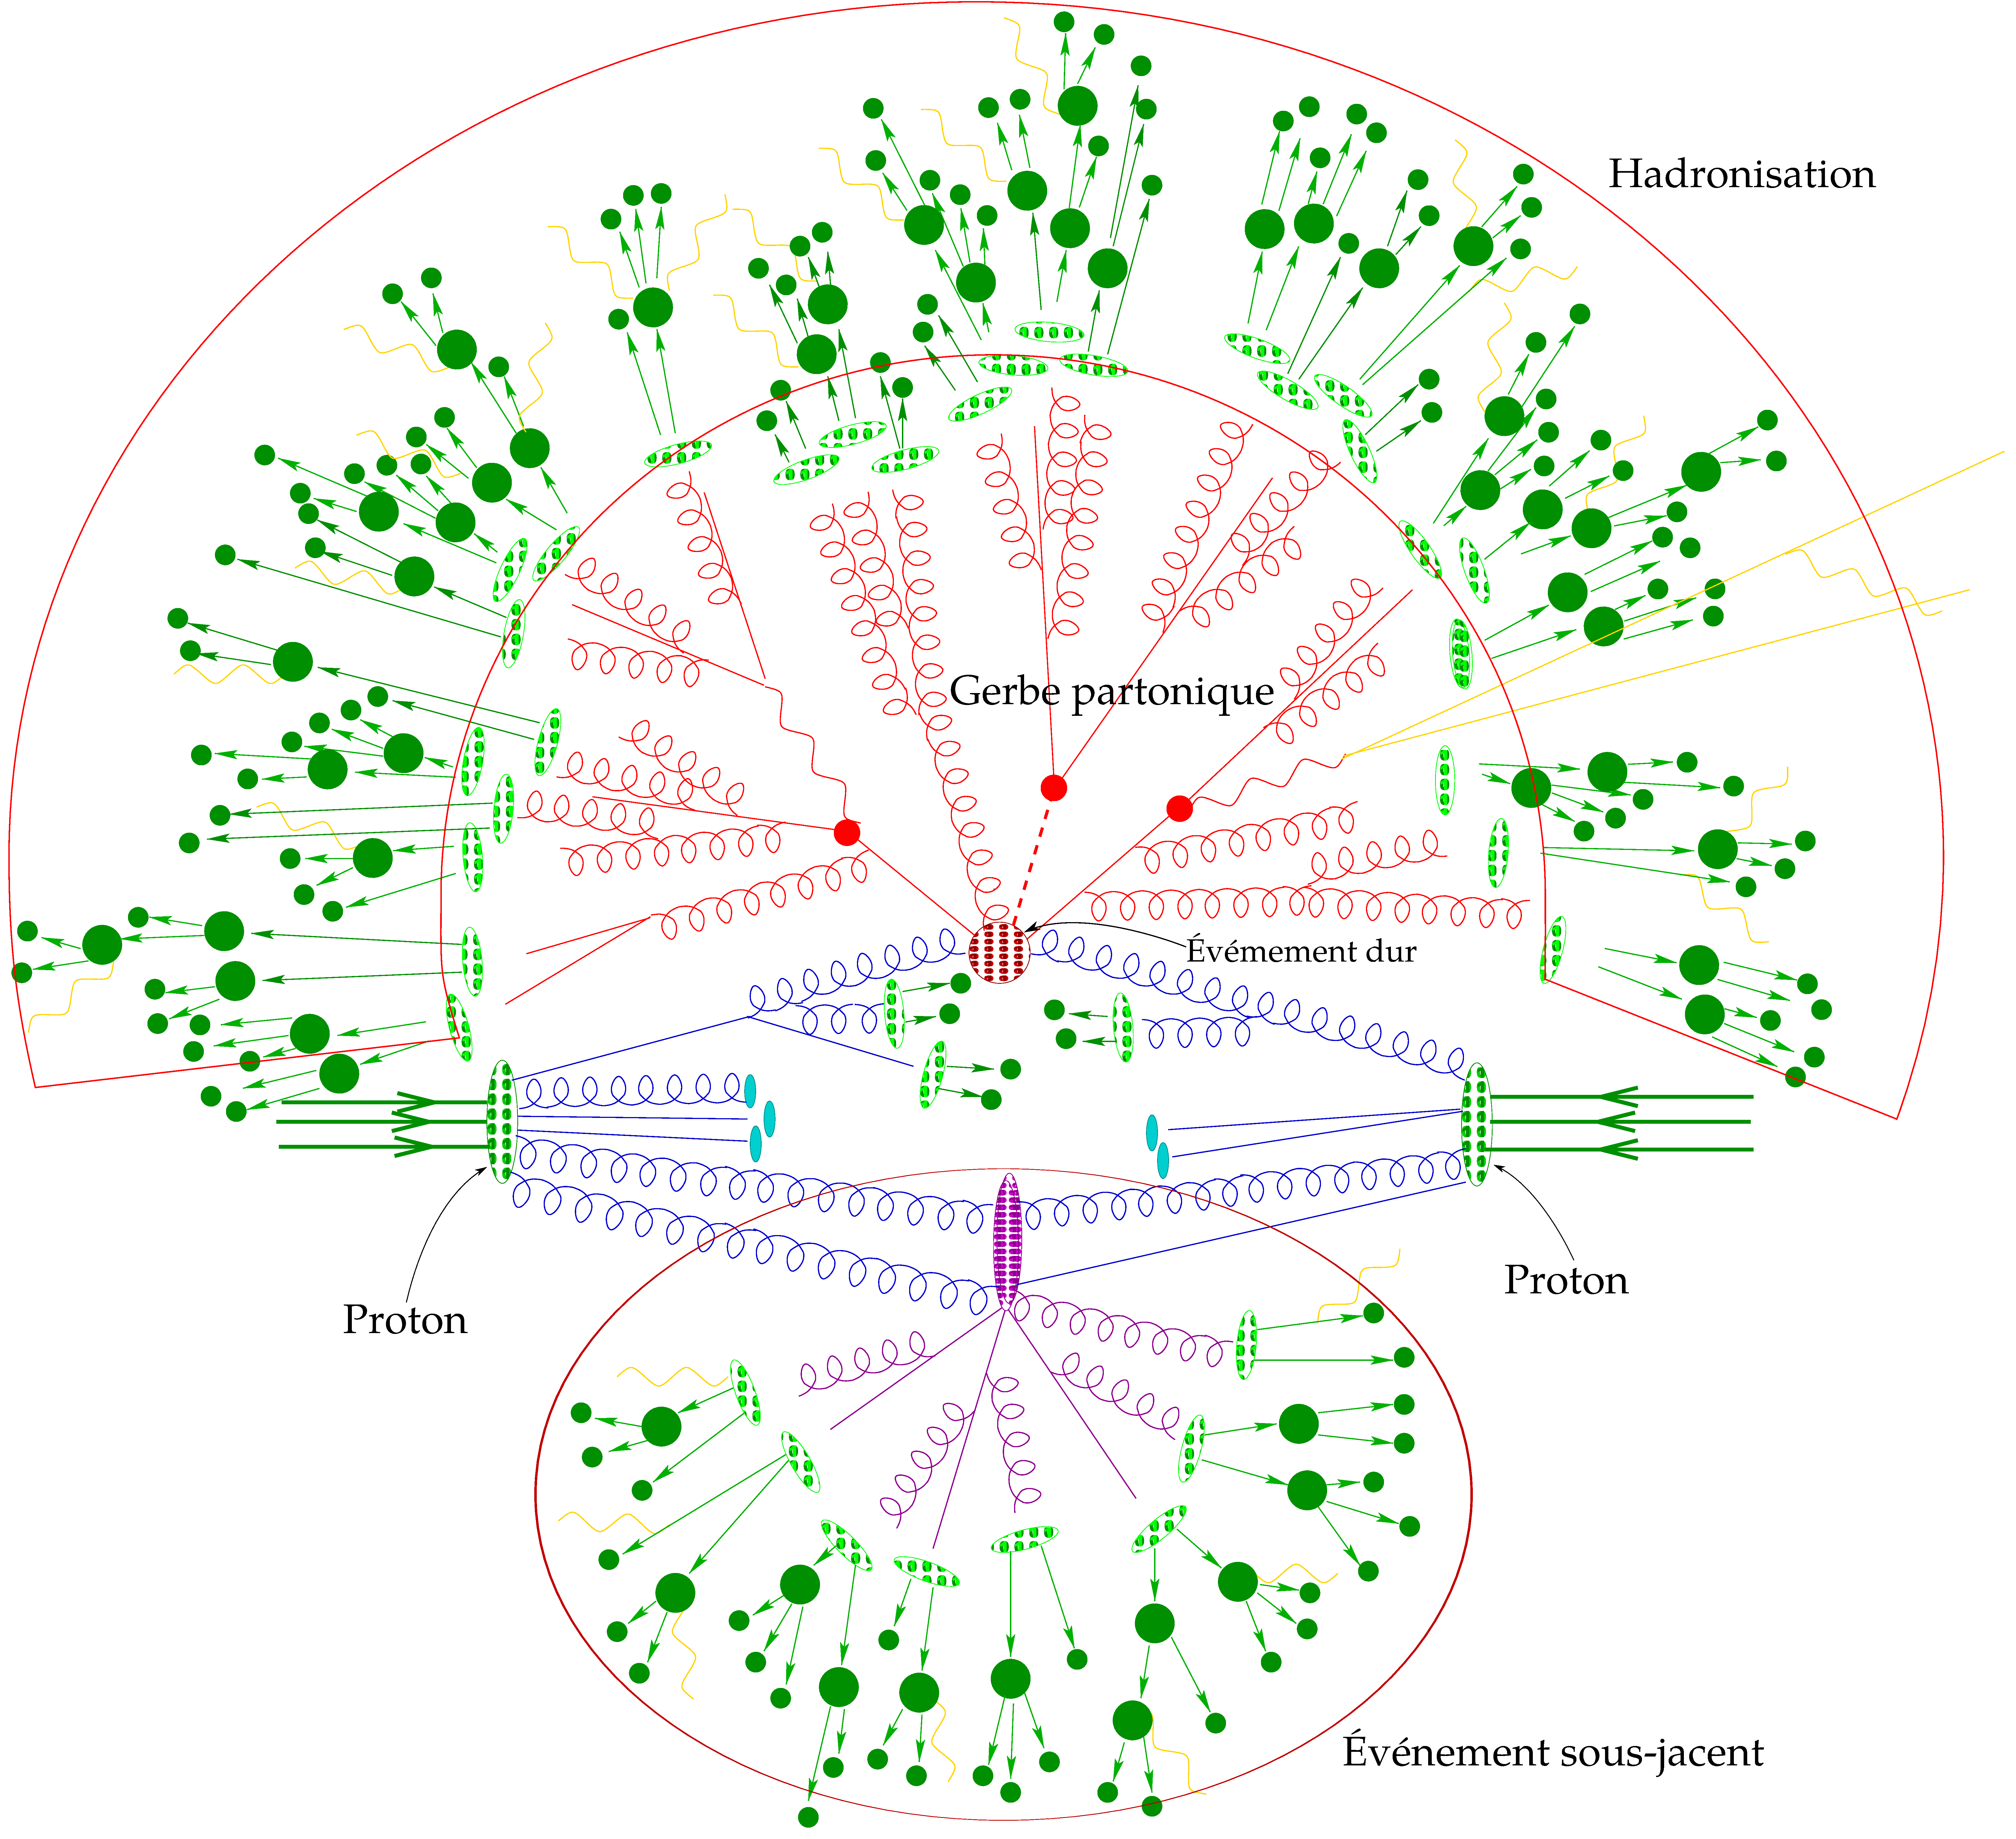
\includegraphics[width=0.99\textwidth]{parton_shower_legend.pdf}
        \caption{Représentation graphique d'une collision de deux protons simulée à l'aide d'un générateur.}
        \label{fig:parton_shower}
    \end{center}
\end{figure}

\subsection{De l'événement dur aux particules dans le détecteur}

Les particules colorées provenant de l'évènement dur génèrent une gerbe partonique. Il s'agit du phénomène de radiation en cascade de particules et de gluons secondaires provenant de gluons de haute énergie. Une fois atteinte une certaine échelle d'énergie, fixée par le générateur, les gluons restants sont forcés de se désintégrer.

Finalement l'hadronisation intervient et ce sont des hadrons neutres du point de vue de l'interaction forte qui sont produits. Ce phénomène se produit environ \SI{5e-24}{\s} après la production de la particule. Il n'existe pas encore de théorie décrivant correctement l'hadronisation, il faut faire appel à des modèles phénoménologiques. 

A l'échelle d'énergie où ils se produisent, la QCD devient non-perturbative, ainsi ses effets sont très complexes à simuler. Il existe néanmoins un ensemble de programmes qui permettent de simuler la chaîne d'hadronisation. On peut citer, par exemple, \texttt{Pythia} \cite{pythia} et \texttt{Herwig} \cite{Corcella:2000bw}. Chacun utilise des algorithmes spécialisés afin de simuler au mieux le développement de la gerbe partonique et de la chaîne d'hadronisation.

\subsection{Simulation du détecteur}

A ce stade, les différentes étapes de générations ont produit une liste de particules stables qui peuvent atteindre le détecteur. Il faut maintenant simuler leurs interactions avec CMS. Cette simulation se compose de :
\begin{itemize}[label=$\triangleright$]
    \item La modélisation du détecteur.
    \item La modélisation des interactions entre particules générées et la matières des sous-détecteurs de CMS (trajectographe, ECAL, HCAL, Chambre à muons)
    \item Les courbures des trajectoires des particules chargées par le solénoïde.
    \item La modélisation de l'empilement.
\end{itemize}

Cette simulation repose sur le logiciel \texttt{Geant\;4} \cite{Agostinelli2003250}. Sa précision va jusqu'à la simulation du câblage interne du détecteur.


\section{Reconstruction des évènements}

\begin{sloppypar}
La simulation du détecteur fournit en sortie les signaux électriques des sous-détecteurs, à l'instar d'une vraie collision. La reconstruction d'un évènement est donc identique lors de la simulation ou d'une prise de données réelle.
\end{sloppypar}

\subsection{L'algorithme \emph{Particle-Flow} (PF)}
\begin{sloppypar}
CMS utilise un algorithme dédié pour reconstruire les objets physiques : l'algorithme du \emph{particle-flow} (PF) \cite{pf,cms_pf_2,cms_pf_jets,cms_pf_leptons, cms_pf_electrons}.
Cet algorithme combine les informations provenant des sous-détecteurs de CMS pour reconstruire les photons, les électrons, les muons, les hadrons neutres et chargés. L'algorithme PF utilise notamment les traces des particules chargées dans le trajectographe, ainsi que les dépôts énergétiques des différents calorimètres. Les particules sont issues d'une interprétation des signatures combinées entre elles. \
\end{sloppypar}

Il doit être noté que l'algorithme possède un taux de fausse identification non nul. Il est ainsi primordial d'avoir la plus haute efficacité de reconstruction possible. Pour maximiser cette efficacité, les sous détecteurs sont pilotés par des algorithmes de trajectographie et de calorimétrie spécialisés.

\subsubsection{Trajectographie itérative} \label{sec:tracks_reconstruction}

Le trajectographe offre une meilleure résolution que les calorimètres pour la mesure de l'impulsion des hadrons. Comme près de \sfrac{2}{3} de l'énergie d'un jet est due à la présence de hadrons chargés, le trajectographe joue un rôle majeur dans la performance du \emph{particle-flow}.

Une procédure itérative \cite{cms_tracks}, basée sur un filtre de Kalman (KF), est utilisé pour reconstruire les trajectoires des particules en minimisant le taux de faux. La graine de cette itération est donnée par la reconstruction induite des \emph{hits} des deux premières couches du détecteur à pixels, ainsi que la position du vertex primaire. La trajectoire est ensuite complétée grâce aux \emph{hits} des autres couches du trajectographe. Les contraintes de cette première étape sont fortes ce qui conduit à un très faible taux de faux. 

Les hits associés à une trajectoire de manière non-ambiguë sont supprimés de la listes des \emph{hits} disponibles. De manière récursive, l'algorithme réitère la construction de trajectoire en relâchant les contraintes à mesure que la liste des \emph{hits} rapetisse. Ainsi, l'efficacité de reconstruction est améliorée tout en gardant un taux de faux très faible grâce à la réduction du nombre de combinaisons.
\begin{sloppypar}
Suite à la troisième itération, on obtient une efficacité de reconstruction de \SI{99.5}{\%} pour les muons isolés et de plus de \SI{90}{\%} pour les hadrons chargés. 
Au-delà, la contrainte sur le point d'interaction est relâchée. Sont ainsi reconstruites les  trajectoires des hadrons chargés secondaires (hadrons provenant de vertex d'interaction déplacé).
\end{sloppypar}
Pour prendre un exemple de reconstruction, une particule chargée de $\pt = \SI{150}{\MeV}$ avec un vertex de production éloigné de plus de \SI{50}{\cm} de l'axe du faisceau, si elle ne laisse que trois \emph{hits}, est reconstruite avec une efficacité de \SI{99}{\%}.

\subsubsection{Vertex d'interaction : reconstruction et empilement}


L'étape suivante est la reconstruction des vertex qui utilisent les traces précédemment reconstruites. On distingue deux étapes : 
\begin{itemize}[label=$\triangleright$]
  \item  Si la différence entre les coordonnées $z$ au point le plus proche de l'axe du faisceau est inférieure à \SI{2}{\mm}, alors les traces sont regroupées en "candidats vertex".
  \item La position du vertex d'interaction est calculée par un algorithme d'ajustement   \cite{Frühwirth:1027031} qui itère sur tous les agrégats de traces. L'algorithme calcule également des indicateurs sur la qualité de l'ajustement ($\chi^2$) en assignant aux traces de l'agrégat un poids variant entre 0 et 1, suivant leur proximité avec l'axe du faisceau.
\end{itemize}

La présence de l'empilement parasite l'évènement dur. Pour outrepasser ce bruit de fond, on identifie le vertex primaire comme celui dont la somme des impulsions transverses en quadrature est la plus grande. Les autres vertex sont utilisés afin de réduire l'impact de l'empilement sur les analyses de physique. En effet, un hadron chargé peut être identifié comme issu de la collision principale ou non, selon le vertex d'interaction auquel sa trace est attachée. On peut alors supprimer du processus de reconstruction tout hadron chargé provenant d'un vertex secondaire que l'on étiquette comme de l'empilement.

\subsubsection{Agglomération calorimétrique}

Le troisième algorithme est l'algorithme d'agglomération calorimétrique de CMS. Il est décomposé en quatre procédures:
\begin{enumerate}
  \item \begin{sloppypar}Mesurer l'énergie des particules neutres (photons, hadrons neutres).
  \end{sloppypar}
  \item Séparer les dépôts d'énergies des particules neutres de ceux des particules chargées.
  \item Reconstruire les photons, les électrons et le rayonnement Bremsstrahlung associé.
  \item Aider à la mesure de l'énergie des hadrons chargés pour lesquels la trajectoire n'a pas été bien reconstruite (hadrons de bas \pt).
\end{enumerate}

Cet algorithme est appliqué de façon séparée dans chaque sous-calorimètre (tonneau du ECAL, tonneau du HCAL, bouchons du ECAL et HCAL, \ldots) en trois phases.

\begin{figure}
  \subcaptionbox{\label{fig:calo_topo}}[0.45\textwidth]{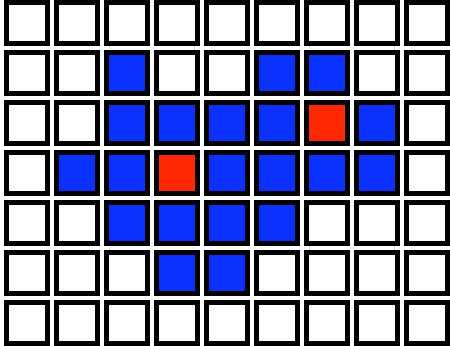
\includegraphics[width=0.45\textwidth]{calo_topoclus_seeds.pdf}}\hfill
  \subcaptionbox{\label{fig:calo_depth}}[0.45\textwidth]{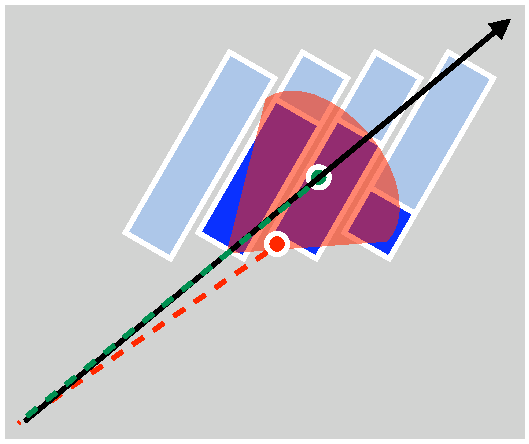
\includegraphics[width=0.45\textwidth]{calo_depthcor.pdf}}
  \caption{Agglomérat topologique contenant deux graines (\subref{fig:calo_topo}) et détermination de la profondeur du dépôt d'énergie (\subref{fig:calo_depth}). En rouge, la position déterminée sans tenir compte de la profondeur biaisée \aeta. En vert, la profondeur est correctement estimée.}
\end{figure}

\begin{description}
\item[Identification des graines] 
\begin{sloppypar}
Il s'agit de repérer les cellules calorimétriques où l'énergie dépasse un certain seuil. Ce seuil est fixé par majoration du bruit de fond du détecteur. Les graines contraignent les cellules voisines à ne pas devenir elles même des graines.
\end{sloppypar}
\item[Definition d'un agglomérat topologique] 
\begin{sloppypar}
Cet agrégat est construit en agrégeant aux graines toutes les cellules qui leur sont adjacentes et possédant une énergie au dessus d'un seuil, fixé comme deux fois la déviation standard du bruit électronique dans le ECAL (\SI{80}{\MeV} dans le tonneau, \SI{\sim 300}{\MeV} dans les bouchons) et à \SI{800}{\MeV} dans le HCAL. Il peut y avoir plusieurs graines dans un même agglomérat topologique. Dans ce cas, le partage de l'énergie entre chaque graine est effectué selon la distance entre la cellule et la graine, en considérant que les gerbes électromagnétiques déposent leur énergie selon un profil gaussien, dont la largeur ne dépend pas de l'énergie. On peut voir une illustration dans la figure \figurename{\ref{fig:calo_topo}}.
\end{sloppypar}
\item[Identification de la position des agglomérats] 
\begin{sloppypar}
La position de l'agrégat est déterminée à partir de la graine et des 4 ou 8 cellules voisines, à l'aide de la formule:
\begin{equation*}
  X = \frac{ \sum_i{w_i X_i} }{ \sum_i{w_i} }\text{, avec } w_i = \ln{\frac{E_i}{E_{th}}}
\end{equation*}
avec $X = x, y$ ou $z$, $X_i$ la position de la cellule $i$, $E_i$ l'énergie de la cellule $i$, et $E_{th}$ le seuil en énergie. Si l'agrégat ne compte qu'une seule graine, toutes les cellules de l'agrégat sont utilisées pour calculer la position.
 Afin de ne pas introduire de biais en $\eta$ lors de la détermination de la position, on estime la profondeur du maximum de la gerbe électronique par la formule
\begin{equation*}
  p = a\left( b + \ln{E} \right)
\end{equation*}
où $p$ est la profondeur, $a$ et $b$ sont des constantes qui dépendent de $\eta$, et $E$ l'énergie totale de l'agrégat. On peut voir figure \figurename{\ref{fig:calo_depth}} l'effet de cette procédure sur la détermination de la position angulaire de l'agrégat. Une vue géométrique est donnée dans la figure \figurename{\ref{fig:calo_depth}}.
\end{sloppypar}
\end{description} 


\subsubsection{L'algorithme de liaison} \label{sec:pf_links}
La dernière étape est la création du lien entre les traces et les agrégats reconstruits. La subtilité provient du fait qu'une particule peut déposer de l'énergie dans les divers sous-détecteurs. Il faut également éliminer les possibilités de double comptage. Ce dernier algorithme produit des "blocs" d'éléments qui vont ensuite servir la reconstruction des particules. 

Dans un premier temps on extrapole les traces reconstruites dans le trajectographe. On reconstruit la profondeur longitudinale de la gerbe : 
\begin{itemize}[label=$\triangleright$]
  \item Dans le calorimètre électromagnétique, jusqu'à une profondeur correspondant au maximum attendu d'une gerbe électromagnétique.
  \item Dans le calorimètre hadronique, jusqu'à une profondeur d'une interaction nucléaire ($\lambda_0$).
\end{itemize}

Si l'extrapolation passe dans la zone délimitée par l'agrégat alors on relie la trace à l'agrégat. On définit la distance du lien par $\Delta R = \sqrt{\Delta \eta^2 + \Delta  \phi^2}$ dans le plan ($\eta$, $\phi$).
Les électrons émettent un rayonnement Bremsstrahlung, il perdent donc de l'énergie. Pour collecter l'énergie perdue, des trajectoires tangentes à la trajectoire principale sont extrapolées dans le ECAL. 
De la même manière on peut construire un lien entre les deux calorimètres (ECAL et HCAL) par recouvrement de zone.
Finalement, le spectromètre à muons reconstruit aussi des traces. Lorsque l'ajustement entre les traces des chambres à muons et celles du trajectographe donne un $\chi^2$ acceptable, un lien est fait. Le muon est dit global.



\subsubsection{Reconstruction des muons} \label{sec:muon_reco}

Durant les étapes dites de reconstruction des particules, la reconstruction du muon\cite{cms_muons_reco} est la première étape et ce, même avant la reconstruction de l'évènement grâce à l'algorithme du \emph{particle-flow}. Les muons laissent des traces dans le trajectographe et dans les chambres à muons, on a avec eux deux types de reconstructions.


\begin{description}
    \item[Reconstruction des muons globaux]
     \begin{sloppypar}
     Cette reconstruction orientée pour les muons de grande impulsion transverse ($\pt \gtrsim \SI{200}{\GeV}$) consiste en l'interpolation d'un lien entre une trace dans le spectromètre à muons et une trace correspondante, par extrapolation, imprimée dans le trajectographe. L'algorithme de lien trajectoire présenté dans la section \ref{sec:pf_links} fonctionne avec un algorithme similaire. Cette méthode permet d'améliorer la résolution de l'impulsion par rapport à celle utilisant uniquement la trace du trajectographe.
     \end{sloppypar}
    \item[Reconstruction des \emph{tracker} muons] 
        \footnote{Il s'agit de muons qui possède des traces dans le trajectographe mais uniquement un segment de trace dans les chambres.}
    \begin{sloppypar}
        Dans le cas de faibles impulsions ($\pt \lesssim \SI{5}{\GeV}$), cette méthode est préférée.
        L'idée est de ne considérer que les traces présentes dans le trajectographe comme possibles candidats muons. En prenant en compte les pertes d'énergie et l'incertitude due aux multiples diffusions, ces muons sont peu énergétiques. On ne va donc  exiger qu'au minimum une petite trace dans le spectromètre à muons, composée de quelques \emph{hits} de DT ou CSC. Dans le contexte des faibles impulsions, cette approche est plus performante que la reconstruction des muons globaux.
    \end{sloppypar}
\end{description}


Seul \SI{1}{\%} des muons ne sont pas reconstruits par l'une ou les deux méthodes précédentes. 
Les traces orphelines dans les chambres à muons sont rangées dans la troisième catégorie des  muons \emph{standalone}.
Les trois catégories de muons sont ensuite regroupées dans une liste de candidats muons. Les candidats muons globaux et \emph{tracker} muons qui partagent la même trace du trajectographe sont fusionnés en un seul candidat.
Une sélection est effectuée sur les candidats muons reconstruits avec l'algorithme standard afin d'identifier les muons \emph{particle-flow}.
A CMS, on classe les sélections dans trois familles différentes : "isolé", "\emph{pf-tight}" et "\emph{pf-loose}".

\begin{description}
\item[Muon isolé]
\begin{sloppypar}
Les muons sont considérés isolés si, dans un cône de taille $\Delta R = \num{0.3}$ centré sur le muon, la somme du \pt des traces et des agrégats calorimétriques est inférieure à \SI{10}{\%} de l'impulsion du muon. En demandant aux muons d'être également globaux, une grande efficacité est obtenue due à la propreté de l'environnement immédiat autour du muon, l'effet du \emph{particle-flow} est limité.
\end{sloppypar}
\item[Muon \emph{pf-tight}]
\begin{sloppypar}
Cette sélection est optimisée pour identifier les muons au sein des jets. Elle requiert un certain nombre de \emph{hits} dans les traces du spectromètre à muons. Est exigée également une compatibilité entre les dépôts d'énergies dans les calorimètres et ceux obtenus par des simulations.
\end{sloppypar}
\item[Muon \emph{pf-loose}]
\begin{sloppypar}
Cette sélection relâche la contrainte sur le nombre de \emph{hits}, et supprime la contrainte sur les dépôts d'énergie.
\end{sloppypar}
\end{description}

On retire ensuite de la liste des blocs \emph{particle-flow} disponibles, chaque muon reconstruit et on procède ensuite à la reconstruction des électrons.


\subsubsection{Reconstruction des électrons}

Les électrons sont beaucoup plus légers que les muons. Ainsi la radiation Bremsstrahlung est amplifiée par un facteur $\left( \sfrac{m_\mu}{m_e} \right)^4$, ce qui met en défaut l'algorithme de reconstruction des traces de CMS (voir \ref{sec:tracks_reconstruction}). En effet, l'algorithme n'est pas optimisé pour gérer les changement abrupts de trajectoire des électrons, ce qui peut arriver par émission de photon Bremsstrahlung. Uniquement si l'émission est un photon de basse énergie, on peut espérer une reconstruction mais au prix d'une grande incertitude et d'un $\chi^2$ grand.
CMS a développé un algorithme dédié à la résolution de ce problème \cite{pf,cms_pf_leptons,cms_pf_electrons}. 
L'algorithme GSF (pour \emph{Gaussian Sum Filter}) est capable de suivre les brusques changements de trajectoire grâce à son grand nombre de paramètres libres (plus d'une dizaine) et procure ainsi une bien meilleure estimation de l'impulsion des électrons. En contre-partie, cet algorithme est très gourmand en ressource (environ \SI{200}{\ms} par trace), et ne peut donc être utilisé que sur un nombre réduit de traces. Doit donc être introduite une pré-sélection.

Dans l'hypothèse d'un Bremsstrahlung négligeable, l'algorithme GSF reconstruit une trace et l'associe avec un bloc \emph{particle-flow}. Si $E/p \simeq 1$, la trace est sélectionnée.

Au contraire pour un rayonnement Bremsstrahlung trop important, sont distingués deux effets :
\begin{itemize}[label=$\triangleright$]
    \item L'algorithme de reconnaissance de traces échoue lors d'un changement abrupt de trajectoire. La trace résultante contient alors un petit nombre de \emph{hits}.
    \item L'algorithme de reconnaissance de traces reconstruit une trace, mais le $\chi^2$ associé est grand.
\end{itemize}

Une sélection est appliquée en utilisant le nombre de \emph{hits} et le $\chi^2$. Après une interpolation GSF de seulement 5 paramètres libres (donc moins contraignante), le $\chi^2$ est associé avec le rapport $\chi^2_{KF} / \chi^2_{GSF}$, le nombre de \emph{hits} et le facteur de qualité du lien entre le dépôt d'énergie entre le ECAL et la trace en entrée d'un algorithme d'arbres de décision boosté. 

Le candidat est  considéré comme un électron si la sortie de l'algorithme est supérieure à une valeur donnée \cite{cms_pf_electrons}. On retire ensuite les électrons reconstruits de la liste des blocs \emph{particle-flow} disponibles pour la suite de l'algorithme.



\subsubsection{Reconstruction des photons et hadrons neutres}

A ce stade, il ne reste plus que les blocs \emph{particle-flow} correspondants aux hadrons (chargés ou neutres), ainsi qu'aux photons.
En préambule de la reconstruction, les liens crées par l'algorithme de liaison sont simplifiés. Si une trace est liée à plusieurs agrégats dans le HCAL, seul le lien ayant la plus petite distance ($\Delta R$, voir \ref{sec:pf_links}) est gardé. On procède de façon identique pour les liens dans le ECAL.

L'énergie des agrégats calorimétriques liés à une trace peut être très inférieure à l'impulsion de celle-ci, dans moins de \SI{0.3}{‰} des cas. L'hypothèse de la présence d'un muon, ou d'une fausse trace, est privilégié si cette différence est supérieure à $3\sigma$. Un algorithme spécialisé de  reconstruction des muons permet d'identifier ces muons. La trace est considérée comme fausse et est supprimée des blocs \emph{particle-flow} s'il n'y pas de présence de muon. Chaque trace restante donne lieu à la création de hadrons chargés \emph{particle-flow}, dont l'impulsion et l'énergie sont mesurées directement depuis la trace. La reconstruction des jets possède sa propre section \ref{sec:jet_reco}, plus détaillée.

Finalement, il ne reste que les blocs \emph{particle-flow} qui n'ont aucune trace liée. Les photons \emph{particle-flow} sont reconstruits à partir des agrégats dans le ECAL et les  hadrons neutres \emph{particle-flow} avec les agrégats du HCAL.
\newline
 
Pour alléger les notations, les particules \emph{particle-flow} seront simplement appelées particules.




\subsection{Isolation des leptons et des photons}\label{sec:lepton_isolation}

L'isolation d'un lepton (muons et électrons) et des photons est une variable importante dans une analyse. Une particule est dite isolée si dans un cône de rayon donné autour d'elle, l'activité détecteur est faible.
L'isolation relative du lepton est définie par la relation
\begin{align*}
  I_{\Plepton} &= \frac{\sum{\pt^\text{hadrons chargés}} + \sum{\pt^\text{hadrons neutres}} + \sum{\pt^\text{photons}}}{\pt^{\Plepton}}
\end{align*}
où les sommes portent sur les particules contenues dans un cône de rayon $\Delta R$ centré autour du lepton. Ainsi, plus $I$ tend vers 0, plus la particule est isolée. Suivant la saveur du lepton différentes tailles de cônes sont utilisées :
\begin{itemize}[label=$\triangleright$]
  \item $\Delta R = \num{0.4}$ pour les muons
  \item $\Delta R = \num{0.3}$ pour les électrons
\end{itemize}



Pour le calcul de l'isolation, il faut considérer les particules issues de l'interaction principale seulement et éliminer celles provenant de l'empilement. La méthode, appelée CHS, élimine les hadrons chargés issus de l'empilement. Cependant les hadrons neutres étant plus difficilement traitables, on doit appliquer des corrections supplémentaires. Dans le cas des muons, on applique les corrections "$\Delta \beta$" et les corrections de "surface effective" pour les électrons et les photons.

\subsubsection{Corrections $\Delta \beta$}

Une des conséquences de la symétrie d'isospin associée à l'interaction forte est l'apparition d'une relation, dans un premier temps empiriquement découverte, entre l'énergie combinée des hadrons neutres et des photons issus de l'empilement et la moitié de l'énergie totale des hadrons chargées du de l'empilement.
\begin{equation}\label{isolation}
\sum{\pt^\text{hadrons neutres empilement}} + \sum{\pt^\text{photons empilement}} \simeq \num{0.5} \sum{\pt^\text{hadrons chargés empilement}}
\end{equation}
En soustrayant donc cette quantité du calcul d'isolation et en vérifiant la positivité de l'énergie de la partie neutre, on obtient :
\begin{align*}
  I_{\Pmu}^\text{corrigé} &= \frac{\sum{\pt^\text{hadrons chargés}} + \overbrace{\left(\sum{\pt^\text{hadrons neutres}} + \sum{\pt^\text{photons}} - \num{0.5} \sum{\pt^\text{hadrons chargés \pu}} \right)}^{= 0 \text{ si négatif}}}{\pt^{\Plepton}}
\end{align*}
On considère un muon comme isolé si $I_{\Pmu}^\text{corrigé} < \SI{15}{\%}$.



\subsubsection{Corrections à la surface effective}

La stratégie, pour cette correction, est tout d'abord de considérer la partie neutre de l'empilement correspondant à $\rho \times \mathrm{EA}$, où $\rho$ est la densité d'énergie par unité de surface due à l'empilement dans l'évènement calculé avec l'algorithme \texttt{FastJet} \cite{Cacciari_2012} et EA la surface effective :
\begin{equation}
\mathrm{EA} = \frac{\alpha_{I, N_\mathrm{vtx}}}{\alpha_{\rho, N_\mathrm{vtx}}}
\end{equation}
où $\alpha_{I, N_\mathrm{vtx}} $ est la pente de l'isolation définie par l'équation \eqref{isolation} en fonction du nombre $N_\mathrm{vtx}$ de vertex primaires et  $\alpha_{\rho, N_\mathrm{vtx}} $ est la distribution de $\rho$ en fonction du nombre de vertex $ N_\mathrm{vtx}$.

L'isolation corrigée est donc 
\begin{align*}
  I_{\Pe}^\text{corrigé} &= \frac{\sum{\pt^\text{hadrons chargés}} + \overbrace{\left(\sum{\pt^\text{hadrons neutres}} + \sum{\pt^\text{photons}} - \rho\,EA \right)}^{= 0 \text{ si négatif}}}{\pt^{\Plepton}}
\end{align*}
On considère un électron comme isolé si $I_{\Pe}^\text{corrigé} < \SI{6}{\%}$. Cette valeur est plus faible que pour les muons en raison de la taille du cône plus faible également.



\subsection{Reconstruction des jets} \label{sec:jet_reco}

Le confinement lié à l'interaction forte implique que les quarks et gluons produits lors des collisions ne peuvent pas être observés directement. Lors de leur propagation, ils vont se combiner avec d'autres quarks pour former des hadrons. Cette succession d'hadronisations va induire la production d'une gerbe de hadrons. Formée principalement de hadrons, mais aussi de leptons, cette gerbe est appelée \emph{jet}.

On dispose d'une description globale de l'événement, sous forme d'une liste de particules, grâce à l'algorithme de \emph{particle-flow}. On va cependant utiliser des algorithmes spécialisés qui vont parcourir la liste des particules, et former des agrégats suivant certains critères de distance entre les particules, différents selon les algorithmes. A CMS, deux types d'algorithmes sont principalement utilisés : l'algorithme \emph{anti-$k_T$} \cite{antikt} et l'algorithme \emph{Cambridge-Aachen} (C-A) \cite{ca_jets}. L'algorithme utilisé par défaut par la collaboration CMS est \emph{anti-$k_T$}. La figure \figurename{\ref{fig:PFantikt}} montre la composition d'un jet reconstruit avec l'algorithme \emph{anti-$k_T$}. Lorsque que l'on veut étudier la sous-structure au sein d'un jet, c'est ce dernier que l'on va utiliser. Par exemple, dans le cas de la désintégration d'un boson \PW de très grande impulsion, les deux quarks peuvent être produits de façon très colinéaire, entraînant la reconstruction d'un seul gros jet, au lieu de deux.


\begin{figure}
    \begin{center}
    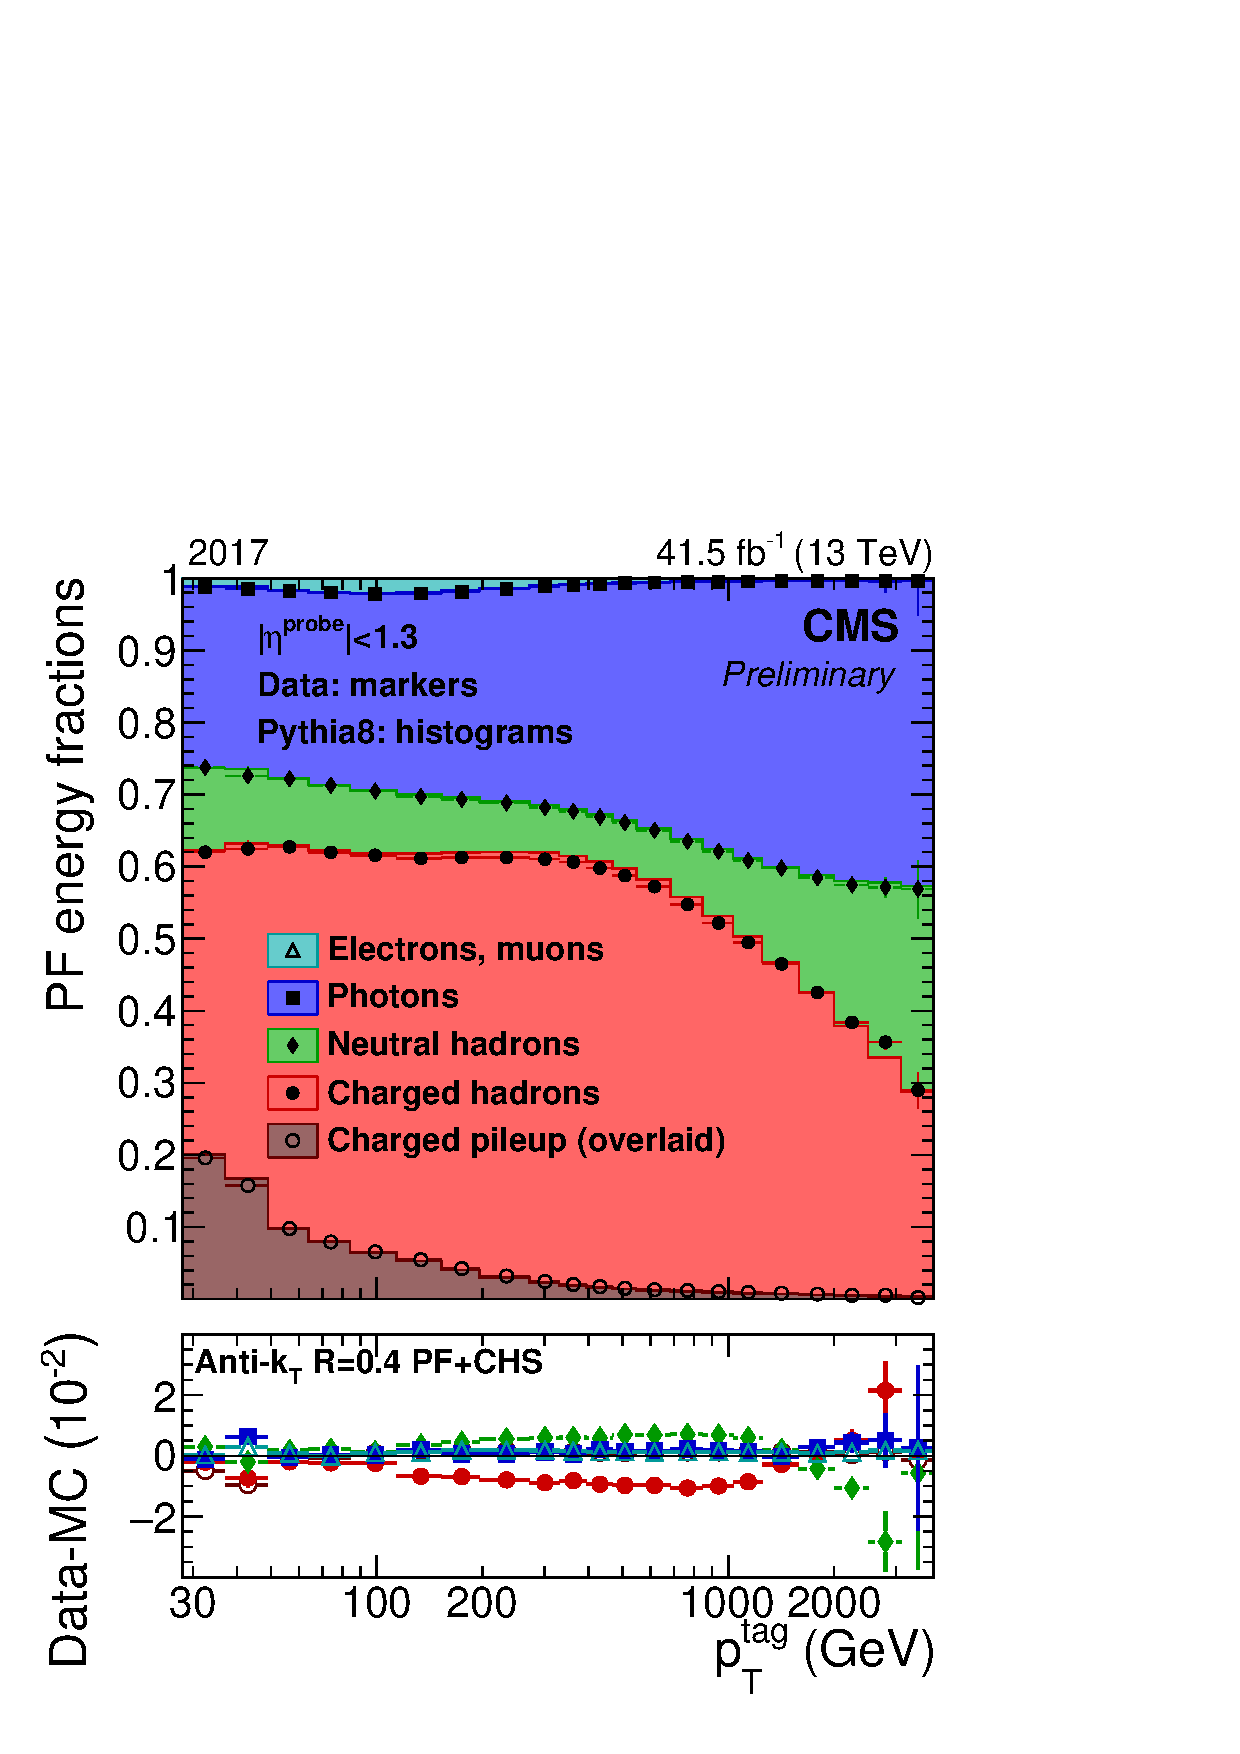
\includegraphics[width=0.5\textwidth]{PF_2017.pdf}
    \caption{Composition des jets reconstruits à l'aide de l'algorithme \emph{anti-$k_T$} en fonction de \pt du jet avec un $\Delta R = 0.4$ dans des évènement dijet sur l’année 2017.}
    \label{fig:PFantikt}
    \end{center}
\end{figure}


En premier lieu, on supprime de la liste des particules les leptons isolés (voir \ref{sec:lepton_isolation}) pour ne pas les agréger au sein d'un jet et produire un double comptage.

Les deux algorithmes itèrent sur la collection de particules, et tentent de construire un jet en associant les particules deux à deux. Pour ce faire, ils utilisent les quantités suivantes :
\begin{align*}
  d_{ij} &= \text{min}\left( k_{T, i}^n, k_{T, j}^n \right) \frac{\Delta R^2_{ij}}{R^2} \\
  d_{iB} &= k^n_{T, i}
\end{align*}
où $k_{T, i}$ est l'impulsion transverse de la particule $i$ par rapport à l'axe du faisceau, $\Delta R_{ij}$ la distance entre $i$ et $j$ dans le plan ($\eta$, $\phi$), et $R$ une distance, choisie par l'utilisateur, symbolisant la largeur du jet. Pour l'algorithme \emph{anti-$k_T$}, on a $n = -2$, tandis que pour C-A, on a $n = 1$. $d_{iB}$ est un estimateur de la distance entre la particule $i$ et le faisceau.


La première étape consiste à estimer la valeur minimum $d_{min}$ entre tous les $d_{ij}$ et $d_{iB}$. Si $d_{ij} = d_{min}$ alors les 4-impulsions des objets $i$ et $j$ sont sommées dans un nouvel objet. Par récursion, on complète la liste. Si le minimum est obtenu pour $d_{iB}$, l'objet $i$ est considéré comme un jet et est enlevé de la liste des particules. L'algorithme s'arrête lorsque toutes les particules au-dessus du seuil \pt minimum ont été agglomérées dans un jet.

\begin{sloppypar}
La différence entre ces deux algorithmes réside dans la fonction de la distance entre particules à grouper. Pour \emph{anti-$k_T$}, le poids de chaque paire est proportionnel à $\text{min}\left( 1 / k^2_{T,i}, 1 / k^2_{T,j} \right)$, ce qui revient à fusionner les particules de grandes impulsions les plus proches en premier. Pour C-A, le poids est uniquement proportionnel à la distance entre les paires : les particules les plus proches sont fusionnées en premier. On peut voir sur la figure \figurename{\ref{fig:akt_ca}} un exemple de reconstruction des jets sur un même événement par les deux algorithmes.
\end{sloppypar}

\begin{figure}
    \centering
    \subcaptionbox{\label{fig:jets_akt}}[0.45\textwidth]{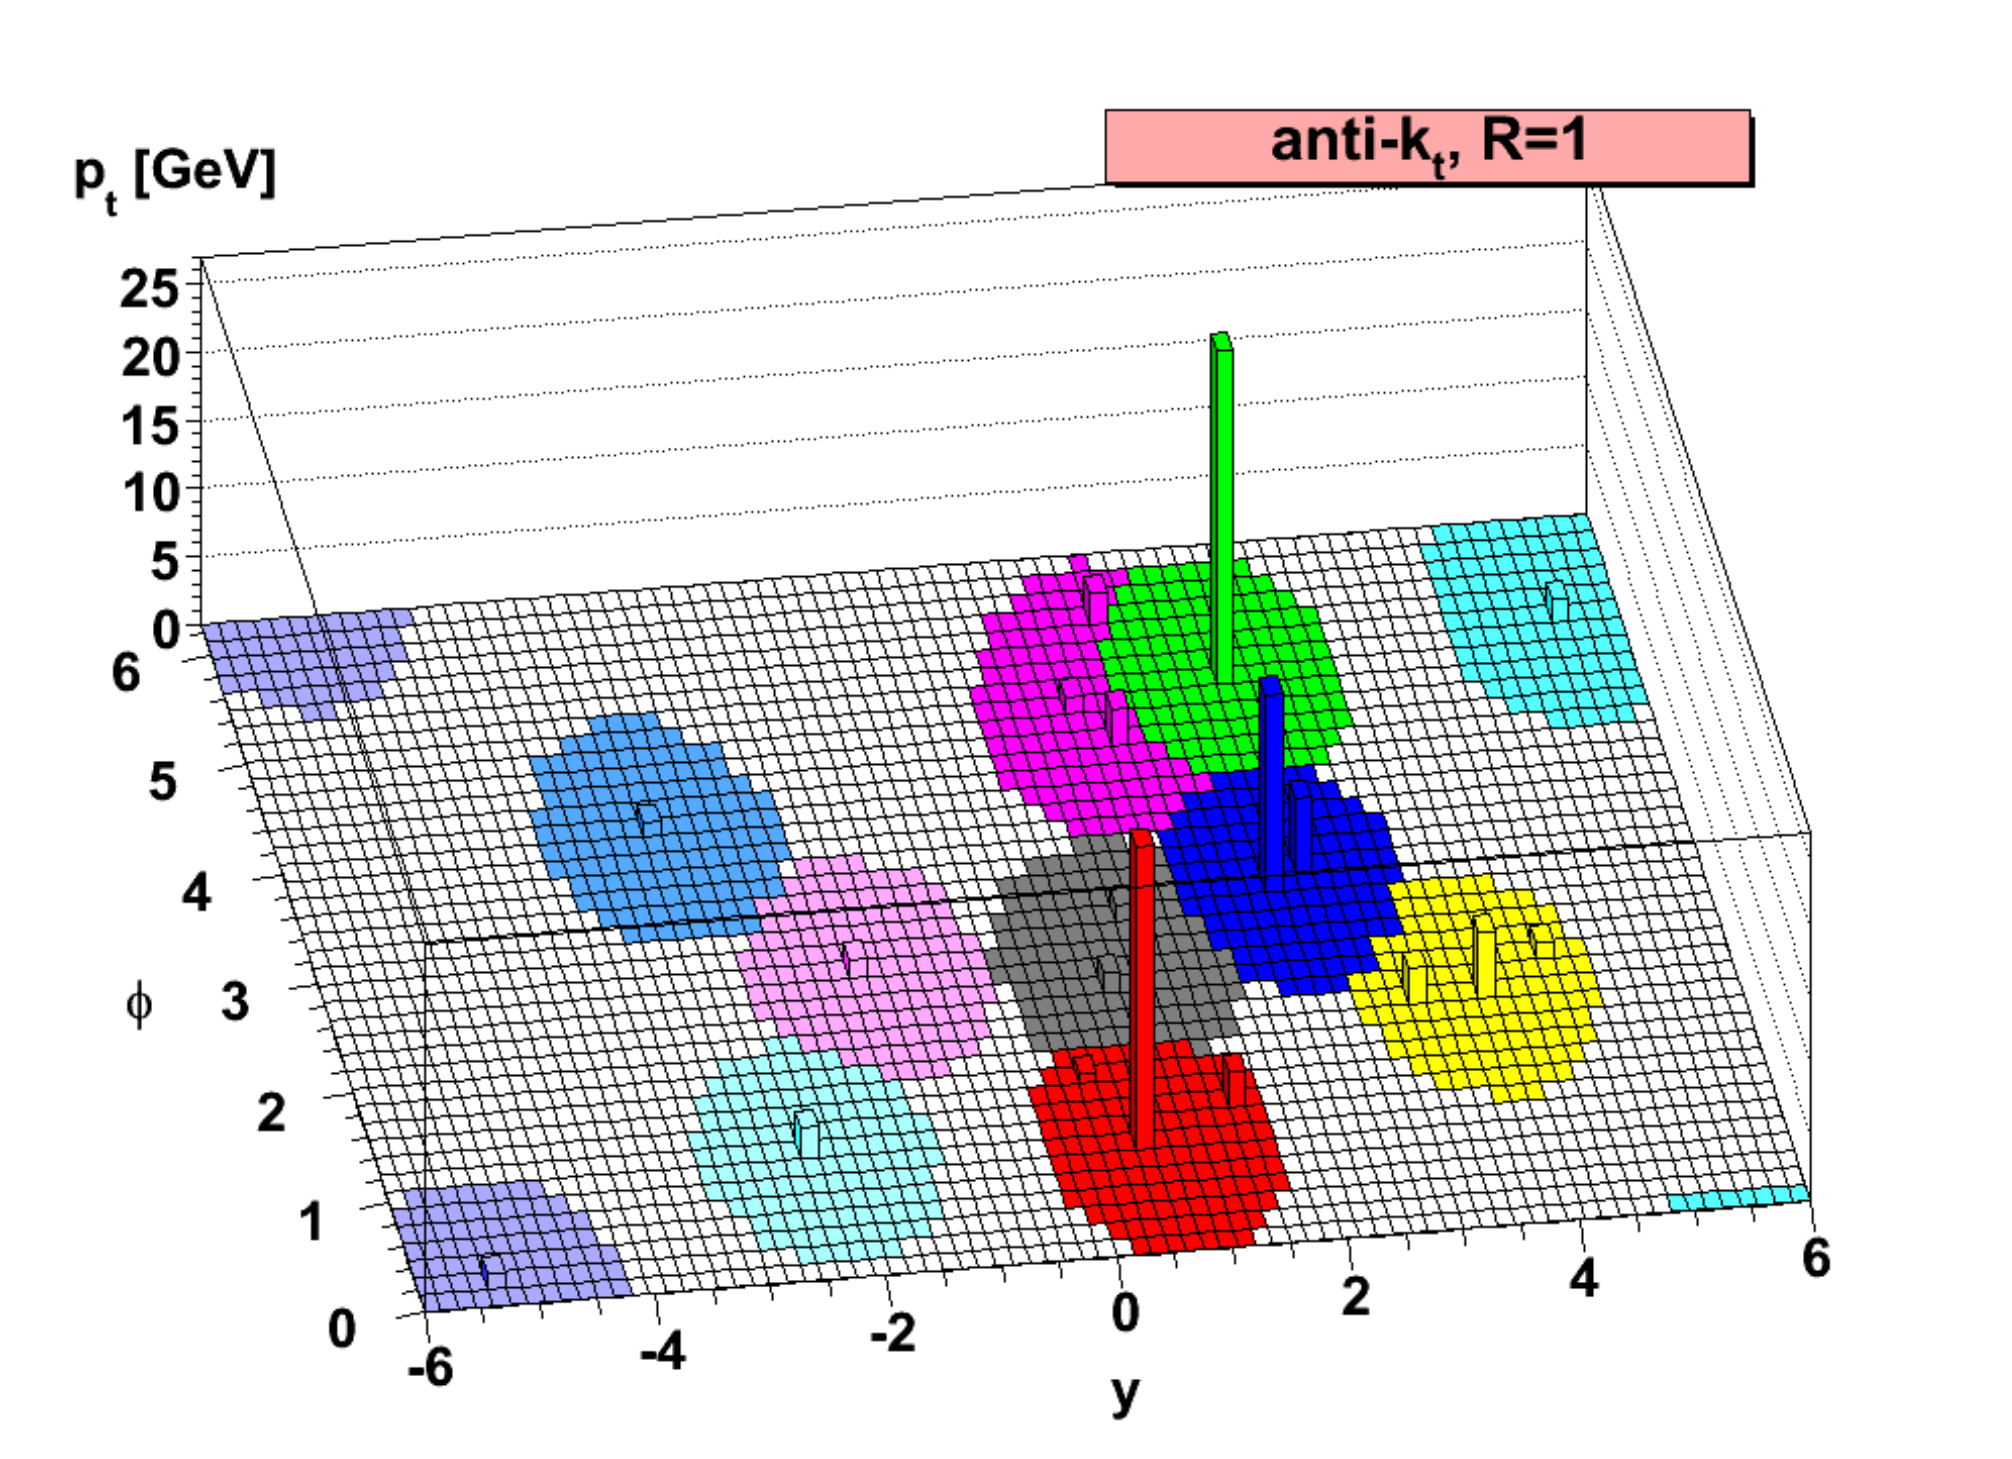
\includegraphics[width=0.45\textwidth]{jets_akt.png}} \hfill
    \subcaptionbox{\label{fig:jets_ca}}[0.45\textwidth]{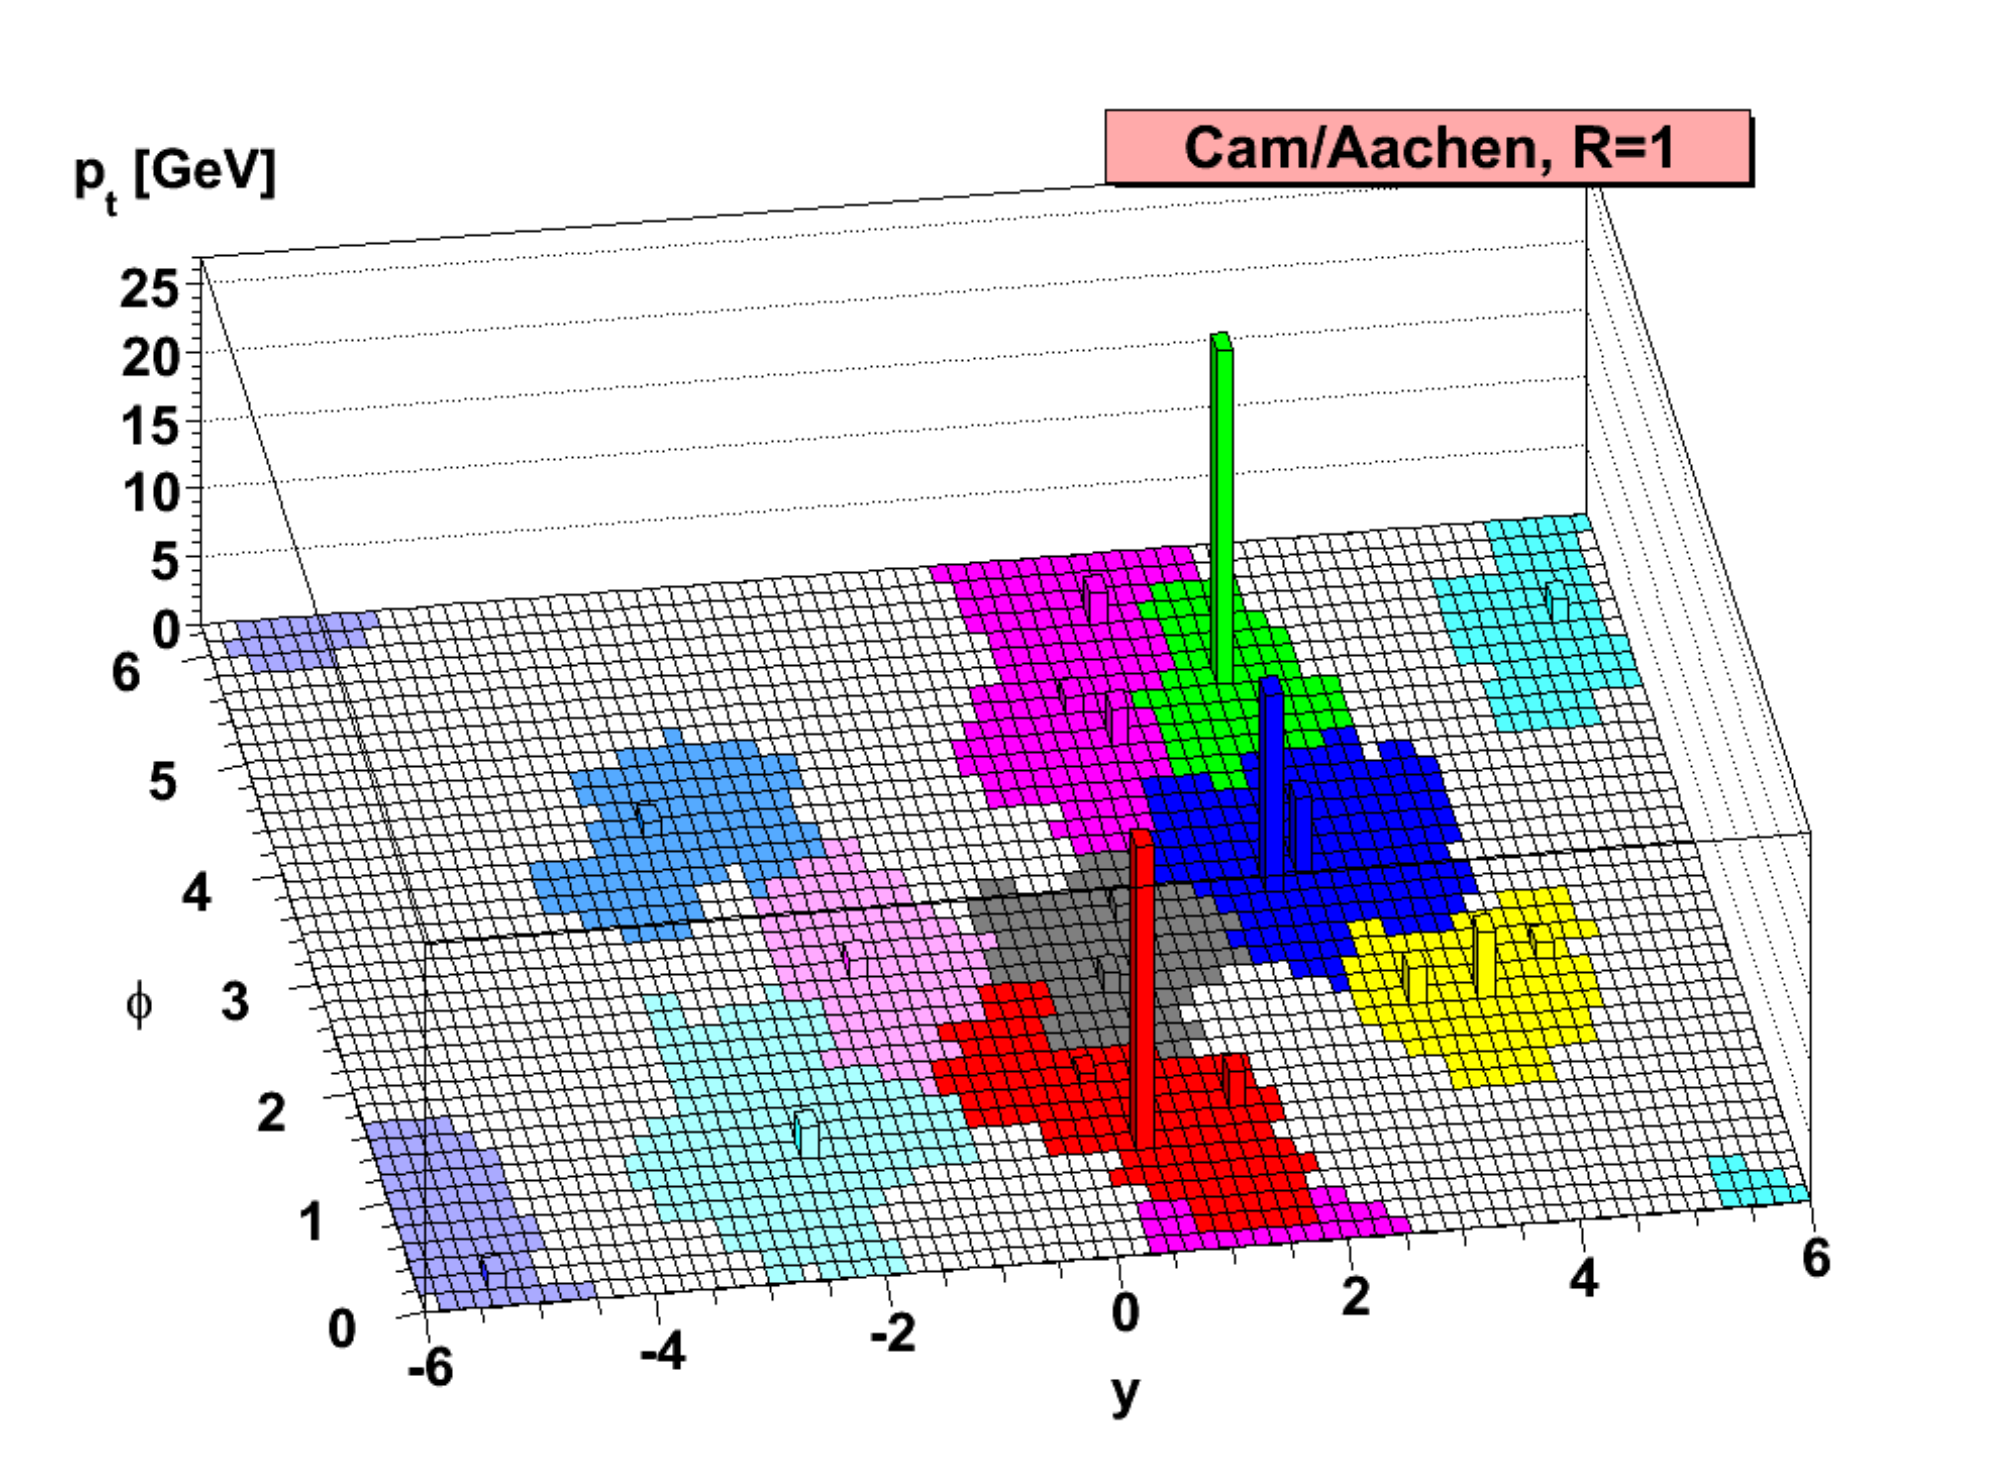
\includegraphics[width=0.45\textwidth]{jets_ca.png}}
    \caption{Reconstruction des jets dans le plan ($\eta$, $\phi$) effectuée sur le même événement par l'algorithme anti-$k_T$ (\subref{fig:jets_akt}) et par l'algorithme C-A (\subref{fig:jets_ca}), pour une distance $R = 1$ \cite{antikt}.}
    \label{fig:akt_ca}
\end{figure}


\subsubsection{Calibration des jets}

Nos algorithmes de reconstruction constituent notre meilleure approximation expérimentale des quarks et des gluons. Il est possible que des particules créées lors de l'hadronisation ne soient pas correctement agglomérées dans le jet. Cela peut être d\^u au fait que ces particules dévient trop de la trajectoire initiale du quark.
De plus, bien que les détecteurs soient étalonnés pour reconstruire au mieux l'énergie des particules, la calibration  reste estimée en moyenne  et ainsi elle impacte la mesure de l'énergie des jets. Les jets doivent donc être étalonnés, c'est-à-dire que leur énergie doit être évaluée au mieux pour correspondre aux simulations avant d'être utilisés dans des analyses physiques.
La résolution en \pt des jets est étudiée après calibration des jets sur des évènements dijet (voir la figure \figurename{\ref{fig:PFantikt}}), $\PZ + \mathrm{jets}$. et $\Pgamma + \mathrm{jets}$.
Des facteurs correctifs sont calculés et fournis centralement au sein de la collaboration, pour tenir compte des différences entre les données et les simulations observées sur les mesures de la résolution \footnote{La résolution des jets obtenus dans les simulations est meilleure que celle des jets reconstruits sur les données.}.




\subsection{Étiquetage des jets issus de quarks $b$} \label{sec:b_tagging}

A CMS, plusieurs algorithmes sont disponibles, permettant d'identifier les jets formés par un quark \Pbottom (\emph{b-tagging}, pour étiquetage des \Pbottom). Nous allons présenter dans cette partie deux algorithmes.

L'algorithme CSVv2 (pour \emph{Combined Secondary Vertex}) permet d'obtenir la probabilité qu'un jet soit de saveur lourde. Cet algorithme consiste en un réseau de neurones dit perception multicouche avec plusieurs couches cachées et un nombre de nœuds correspondant à deux fois le nombre de variables \cite{Sarle94}. Les variables entraînées par le réseau de neurones sont liées au vertex secondaire. On peut noter la masse corrigée du vertex secondaire, nombre de traces liées au vertex secondaire, ... . La liste exhaustive des variables est décrite dans \cite{Sirunyan_2018}. Le réseau est entraîné sur des évènements multijets.
Ils seront ensuite répartis en trois catégories : 
\begin{itemize}[label=$\triangleright$]
\item Un ou plusieurs vertex secondaires ont été reconstruits.
\item Un vertex secondaire n'a pas été reconstruit mais le jet possède au moins deux traces avec un paramètre d'impact 2D d'une significance suffisante ainsi qu'une masse invariante supérieure de \SI{50}{MeV} à la masse du \PKzS.
\item Le reste des évènements.
\end{itemize}

La figure \figurename{\ref{fig:btag_csvv2}}, montre la distribution du discriminant permettant l'identification des jets issus de \Pbottom. Elle est en moyenne plus proche de 1. Cette distribution pour les jets de \Pcharm n'a pas de maximum clair et celui des jets légers est proche de 0. Cet algorithme performant permet une bonne discrimination des jets \Pbottom par rapport aux saveurs légères mais moins par rapport à des jets de \Pcharm.

\begin{figure}
    \centering
    \subcaptionbox{\label{fig:btag_csvv2}}[0.45\textwidth]{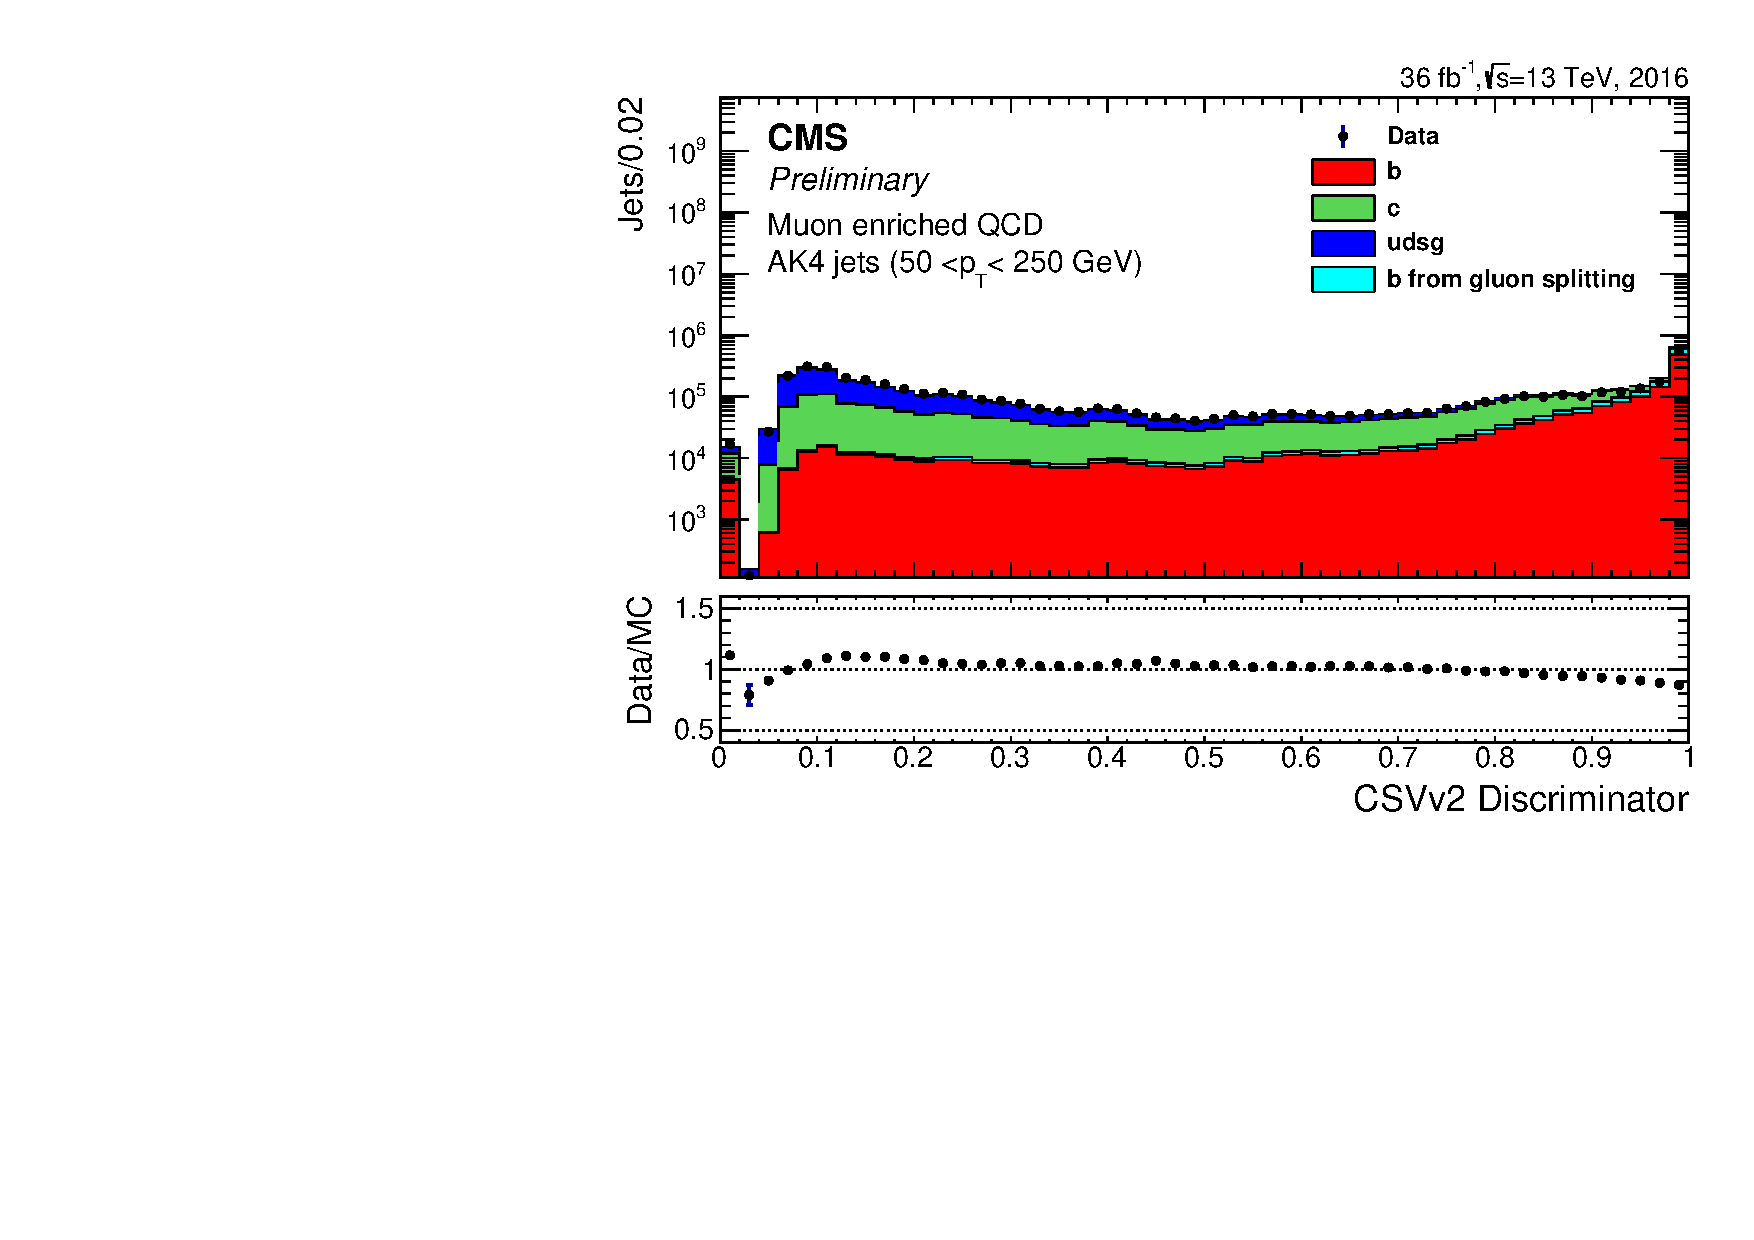
\includegraphics[angle=-90,width=0.45\textwidth]{csvv2jet.pdf}} \hfill
    \subcaptionbox{\label{fig:btag_deepcsv}}[0.45\textwidth]{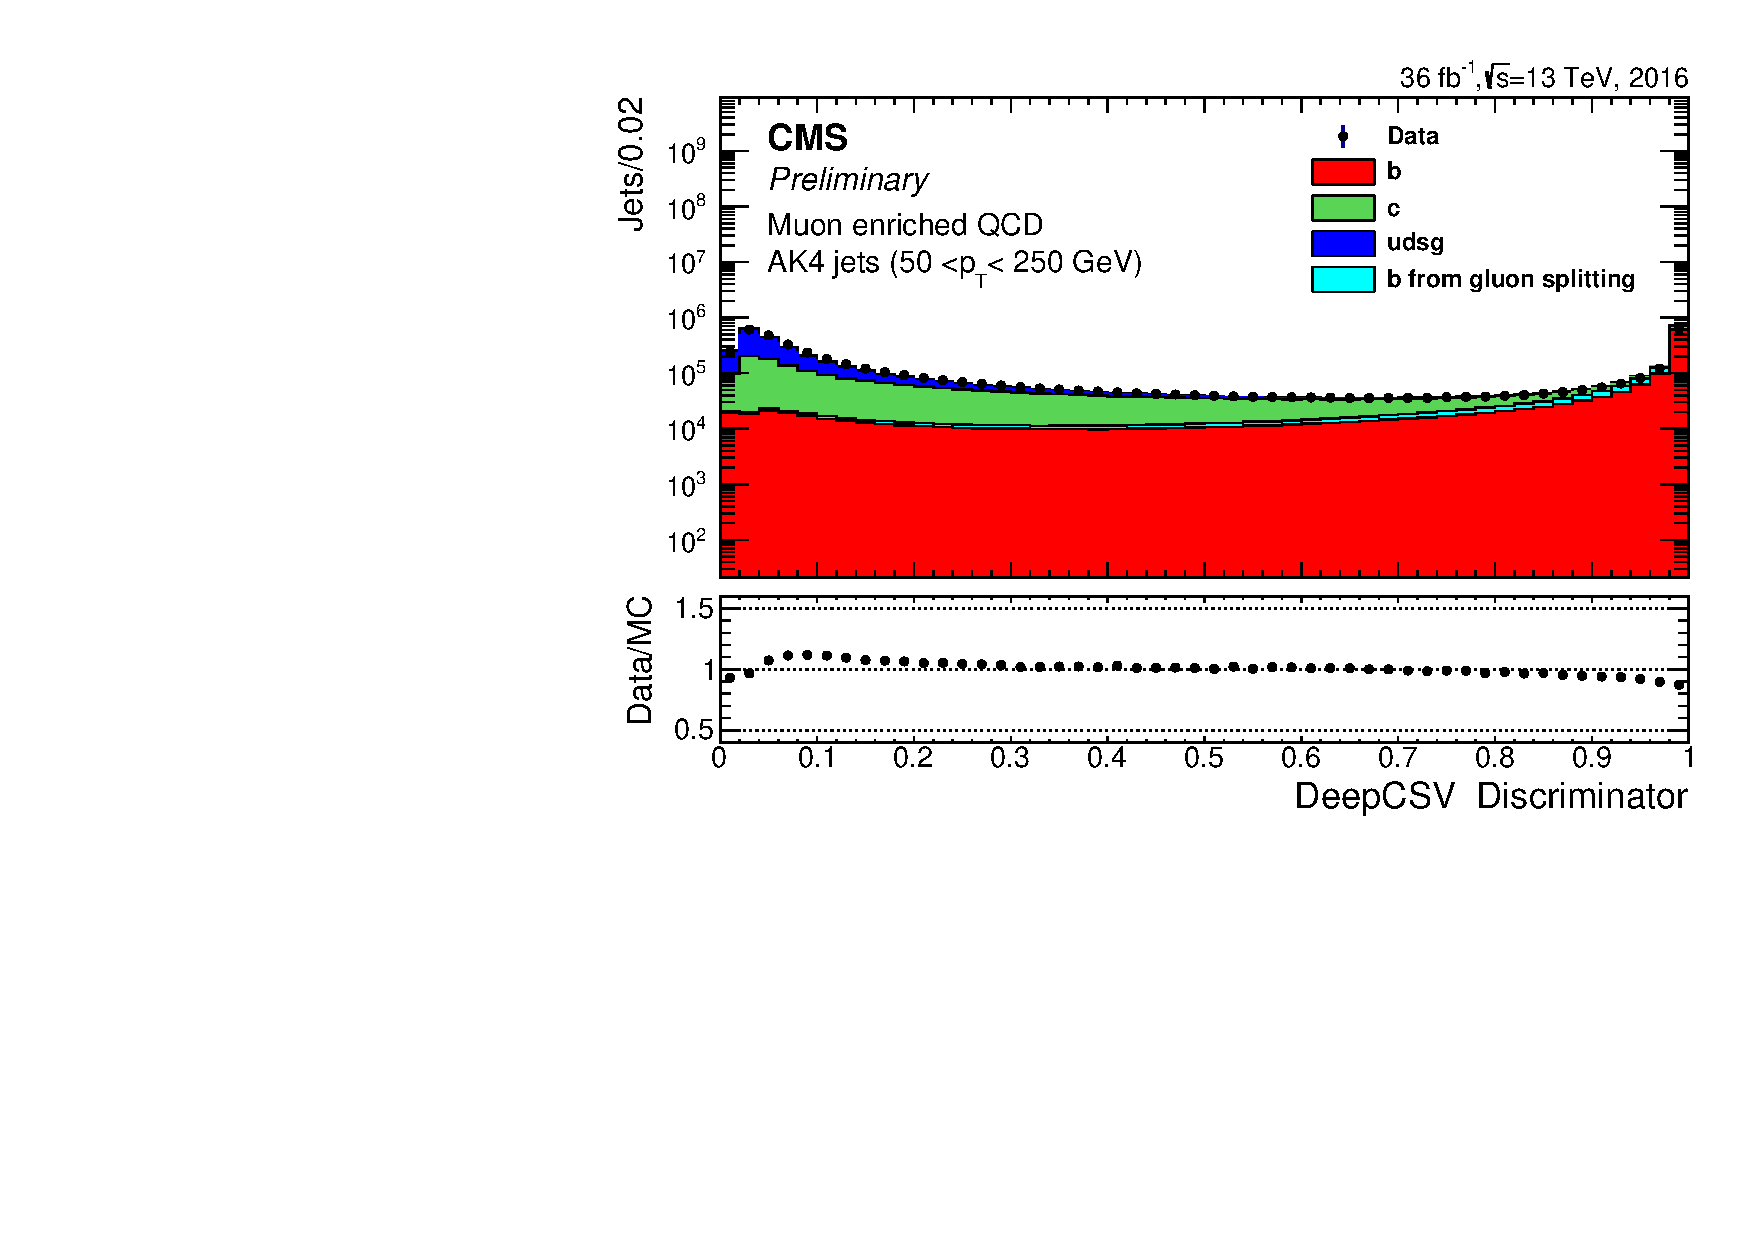
\includegraphics[angle=-90,width=0.45\textwidth]{deepjet.pdf}}
    \caption{Distribution des algorithmes de CSVv2 (\subref{fig:btag_csvv2}) et de DeepCSV  (\subref{fig:btag_deepcsv}).}
\end{figure}

Récemment les avancées de l'apprentissage profond (\emph{deep learning} \cite{Guest_2016}) ont permis l'amélioration des algorithmes. L'algorithme DeepCSV est la version avancée du CSVv2. Cette version comporte quatre couches cachées de 100 nœuds interconnectés. L'entraînement est réalisé sur un mélange \ttbar et multijet. L'architecture du réseau de neurone profond est écrite avec les librairies Kera \cite{chollet2015} et Tensor-Flow \cite{abadi2016}. Le discriminant utilisé pour les jets issus de \Pbottom est présenté à la figure \figurename{\ref{fig:btag_deepcsv}}.

\begin{figure}
    \centering
    \subcaptionbox{\label{fig:perf_log}}[0.45\textwidth]{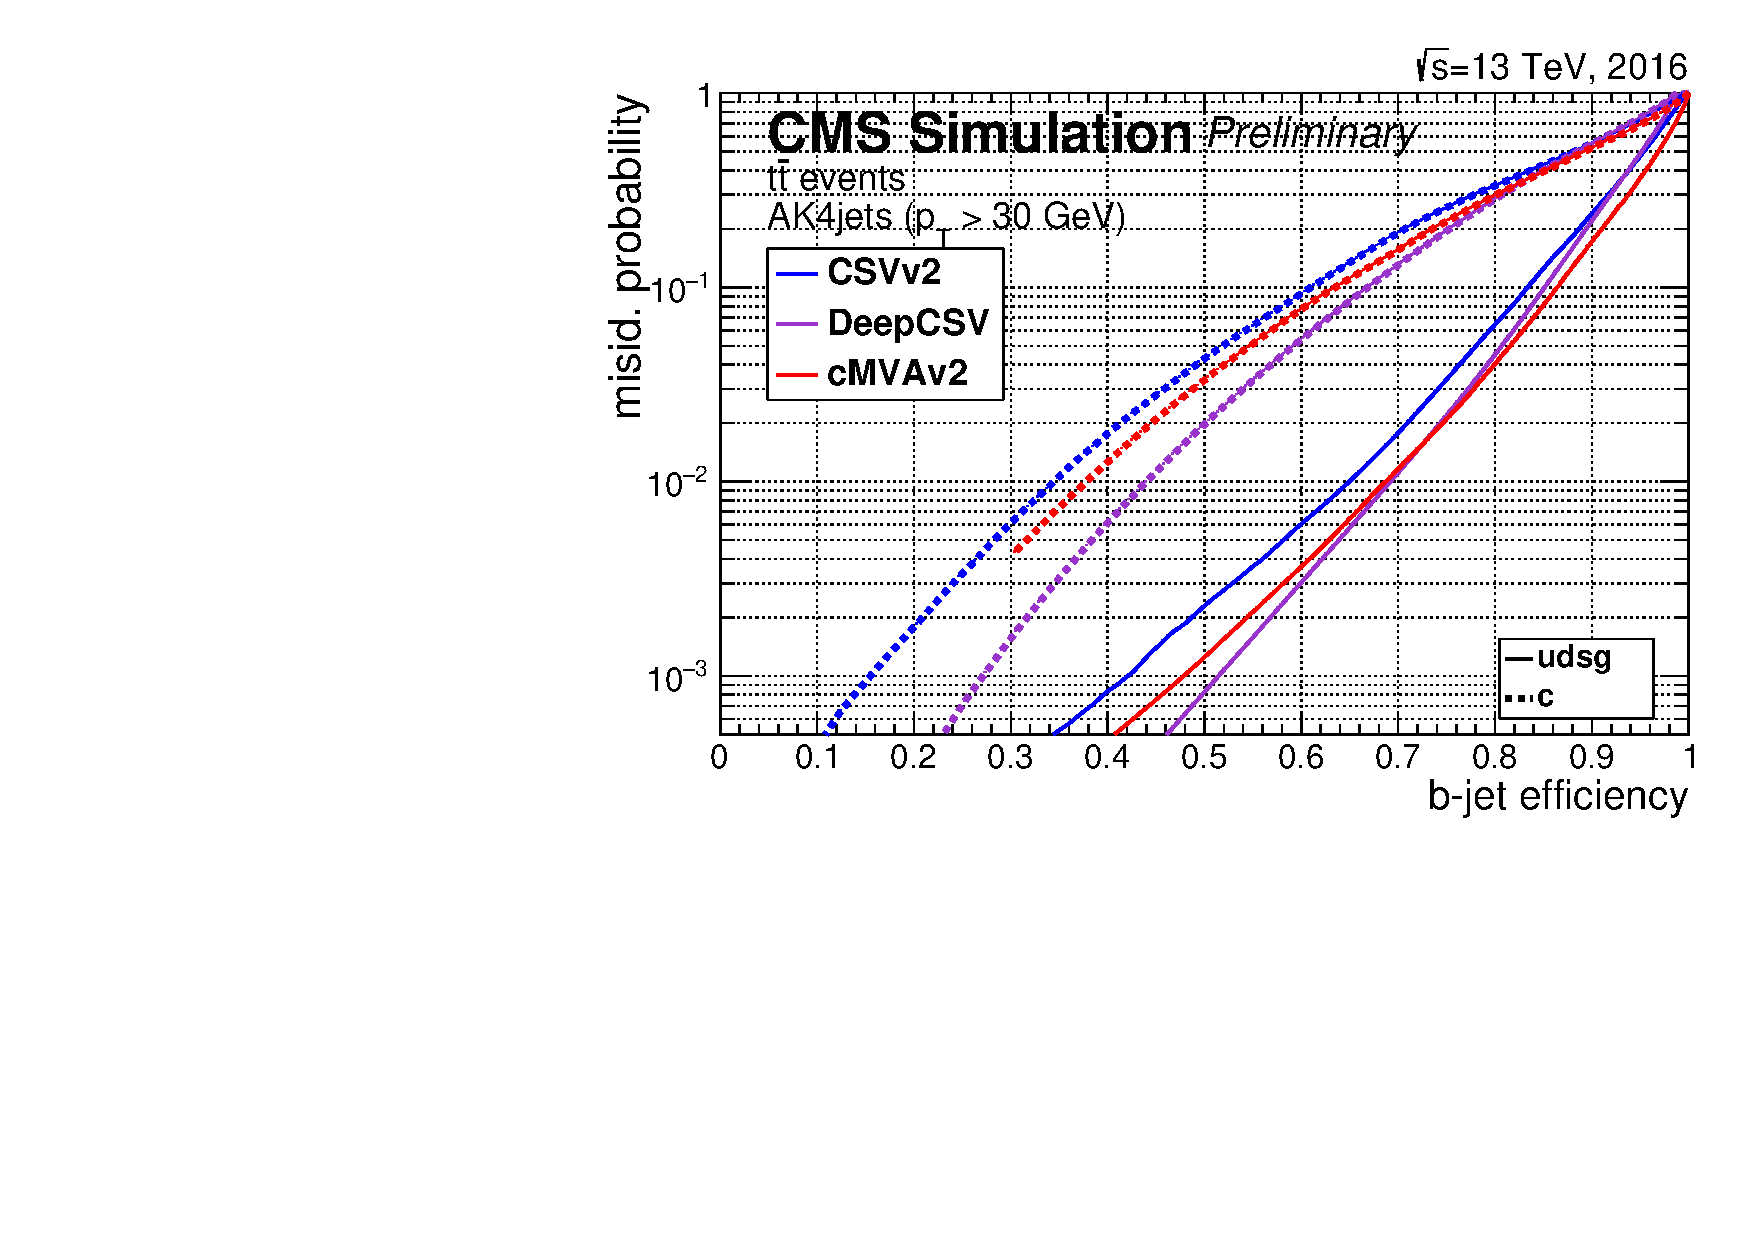
\includegraphics[angle=-90,width=0.45\textwidth]{perf_Log.pdf}} \hfill
    \subcaptionbox{\label{fig:perf_c_log}}[0.45\textwidth]{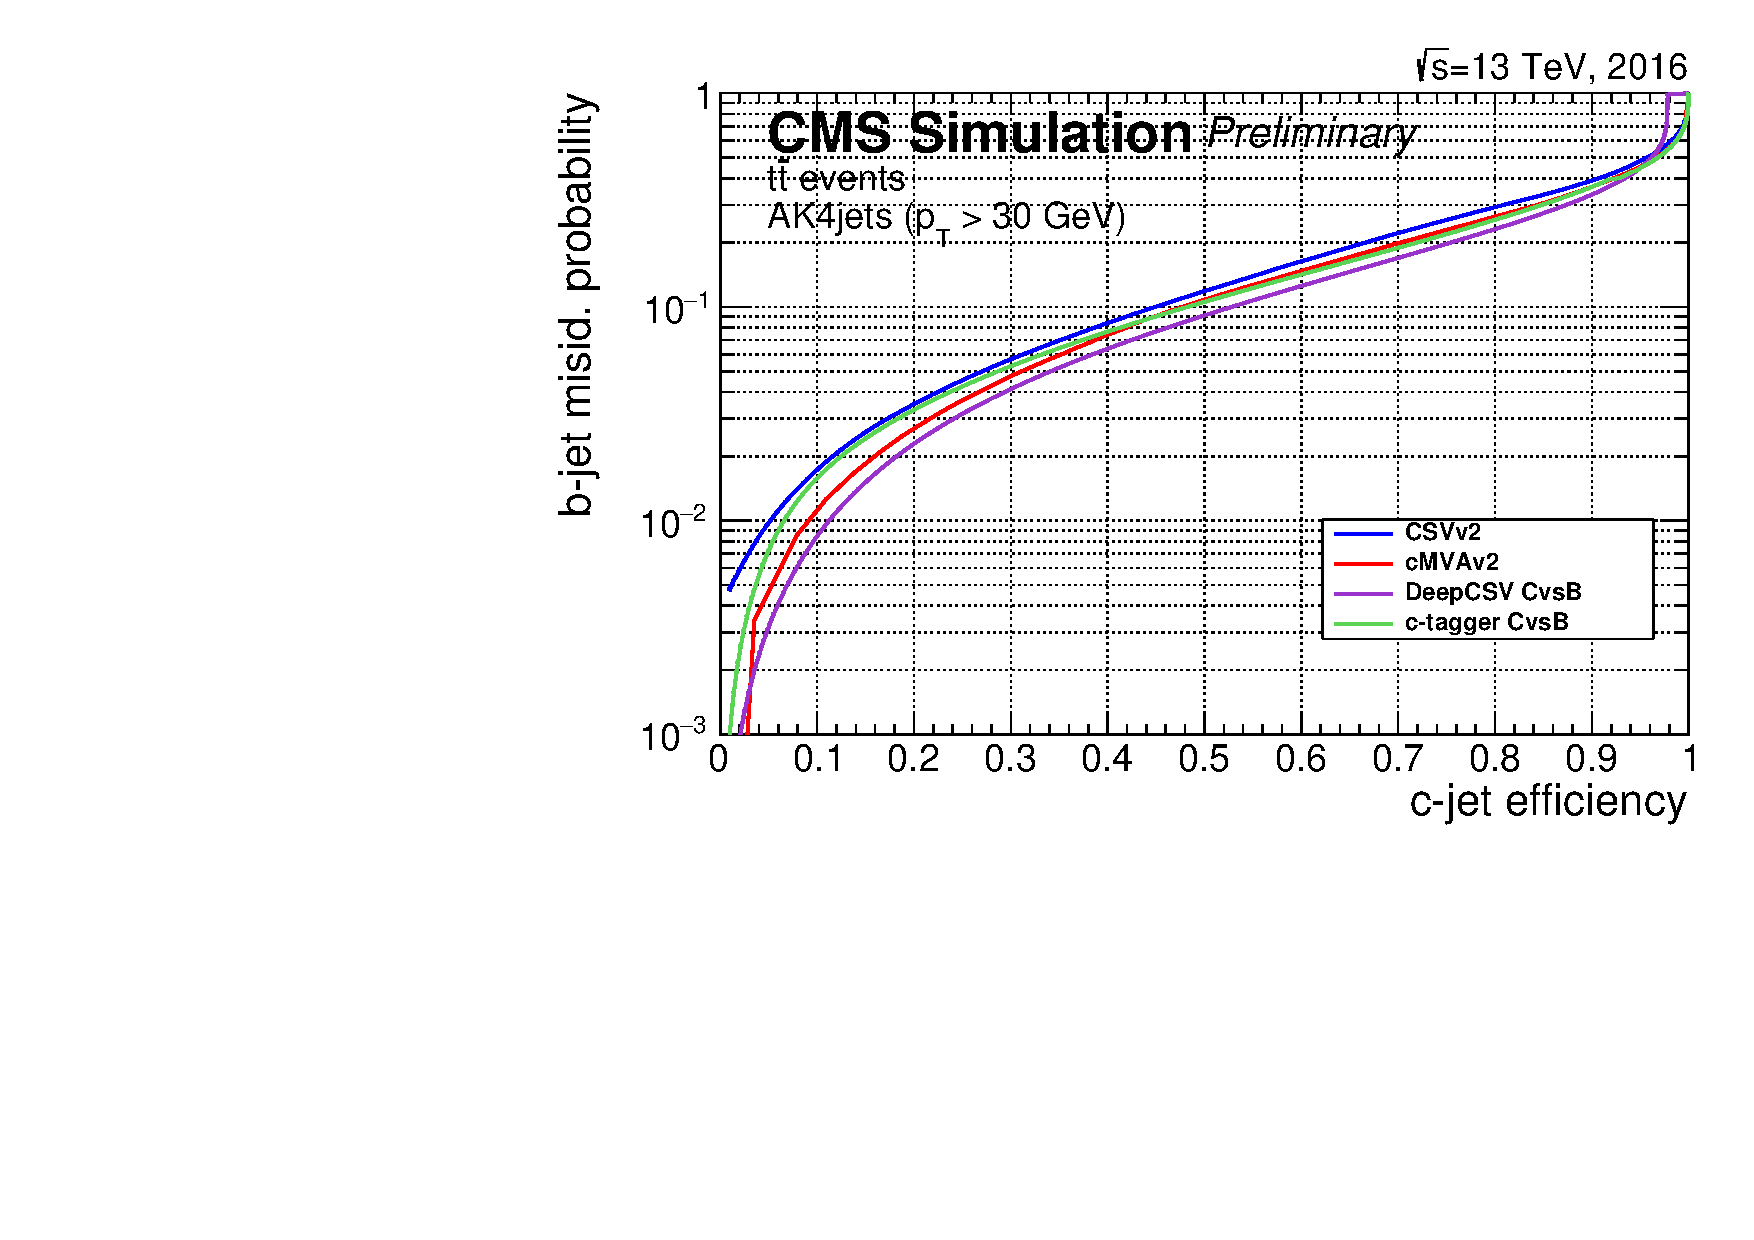
\includegraphics[angle=-90,width=0.45\textwidth]{perf_c_Log.pdf}}
    \caption{Probabilité de mauvaises identifications en fonction de l'efficacité de sélection des jets de \Pbottom (\subref{fig:perf_log}), des jets de \Pcharm (\subref{fig:perf_c_log}) pour différents algorithmes \cite{Sirunyan_2018}.}
\end{figure}

La figure \figurename{\ref{fig:perf_log}} montre la probabilité d'une mauvaise identification d'un jet léger ou d'un \Pcharm comme un jet de \Pbottom en fonction de l'efficacité de sélection des jets de \Pbottom pour les différents algorithmes utilisés dans la collaboration. Cette figure permet de bien choisir son algorithme en fonction des besoins de sa propre analyse.

Les algorithmes d'identification sont entraînés sur des échantillons simulés pour obtenir les meilleures performances possibles et ne pas introduire de biais provenant de différences entre les données et les simulations. Les corrections sont extraites en utilisant la méthode dite de \emph{tag and prob} \cite{Sirunyan_2018} et un ajustement itératif \cite{Khachatryan_2014}. Ces méthodes sont appliquées sur des évènements de données $\PZ + \mathrm{jets}$. Le jet dont la saveur est estimée à l'aide de l'algorithme est utilisé comme étiquette et les autres jets comme des sondes. La distribution du discriminant dans les simulations est normalisée à celle observée dans les données. 


\subsection{Énergie transverse manquante}

Par rapport au repère conventionnel de CMS, les collisions se déroulent le long de l'axe $z$. L'impulsion initiale dans le plan ($x$, $y$) est donc nulle.
Après reconstruction de l'évènement, le bilan doit rester nul en vertu de la conservation de l'impulsion. Un bilan non nul signifie que des particules n'ont pas été correctement reconstruites. Les neutrinos interagissent très peu avec la matière, il ne sont par conséquent jamais détectés et font partie de ces particules non reconstruites. 


Pour quantifier cette perte d'énergie, on introduit le vecteur d'énergie transverse manquante \PTm et l'energie transverse manquante (MET), sa norme, noté \met. A l'aide de l'algorithme de \emph{particle-flow}, on définit le vecteur énergie transverse manquante comme l'opposé de la somme vectorielle des impulsions transverses de toutes les particules de l'événement. La résolution sur la mesure de \met est très importante, puisque de nombreux modèles de nouvelle physique prédisent des particules qui interagissent peu voire pas avec la matière : l'énergie manquante est alors le seul moyen de pouvoir les mettre en évidence.
Dans l'analyse de cette thèse, une résolution précise de \met ne sera pas utilisée car le canal $\ttbar \rightarrow \Pbottom \Pleptonplus \Pnulepton +  \APbottom \Pleptonminus \APnulepton$ a déjà un très bon rapport signal sur bruit  de fond.

\section{Conclusion}

Dans ce chapitre nous avons vu qu'il faut mettre en place une chaîne de simulation complète et performante pour confronter les données aux prédictions théoriques. La première étape de la chaîne est la réalisation d'une simulation physique. Elle comprend les phénomènes de collisions entre partons, radiations de gluons, hadronisation, désintégration des particules instables, l'évènement sous-jacent et les collisions multiples. De plus, une simulation précise du détecteur CMS est nécessaire pour simuler les réponses des différents sous-détecteurs aux particules produites.

Les signaux électriques fournis par le détecteur sont convertis en objets physiques. Le processus de reconstruction est commun aux simulations et aux données. Pour améliorer la résolution des différents objets reconstruits, on utilise l'algorithme \emph{particle-flow} qui combine les informations fournies par les différents sous-détecteurs. On a également vu que plusieurs outils utilisent les résultats du \emph{particle-flow}. Par exemple, l'algorithme de reconstruction des jets qui est central dans l'environnement hadronique qu'est le LHC. Les jets présentent une moins bonne résolution que les muons ou les photons, ainsi d'importantes méthodes de calibrations sont déployées pour une mesure de l'énergie plus précise.

\end{fmffile}